\subsection{Overordnet tilgang}
Tilgangen til projektet er baseret på MUST principperne beskrevet i 'Professionel it-forundersøgelse'. Ligeledes er de benyttede og de fremtidige redskaber og aktiviteter beskrevet i projektgrundlaget baseret på anbefalinger fra samme bog.\\
Nedenfor findes vores udarbejdede baseline som viser deadlines og produkter for vores projekt. Forberedelsesfasen og fokuseringsfasen er blevet lagt sammen, og de aktiviteter beskrevet i denne kombi-fase er blevet udført. Aktiviteterne i de fremtidige faser er foreløbige og stadig til debat hvorvidt de skal ændres.
\begin{figure}[H]
	\hspace{-1.5cm}
	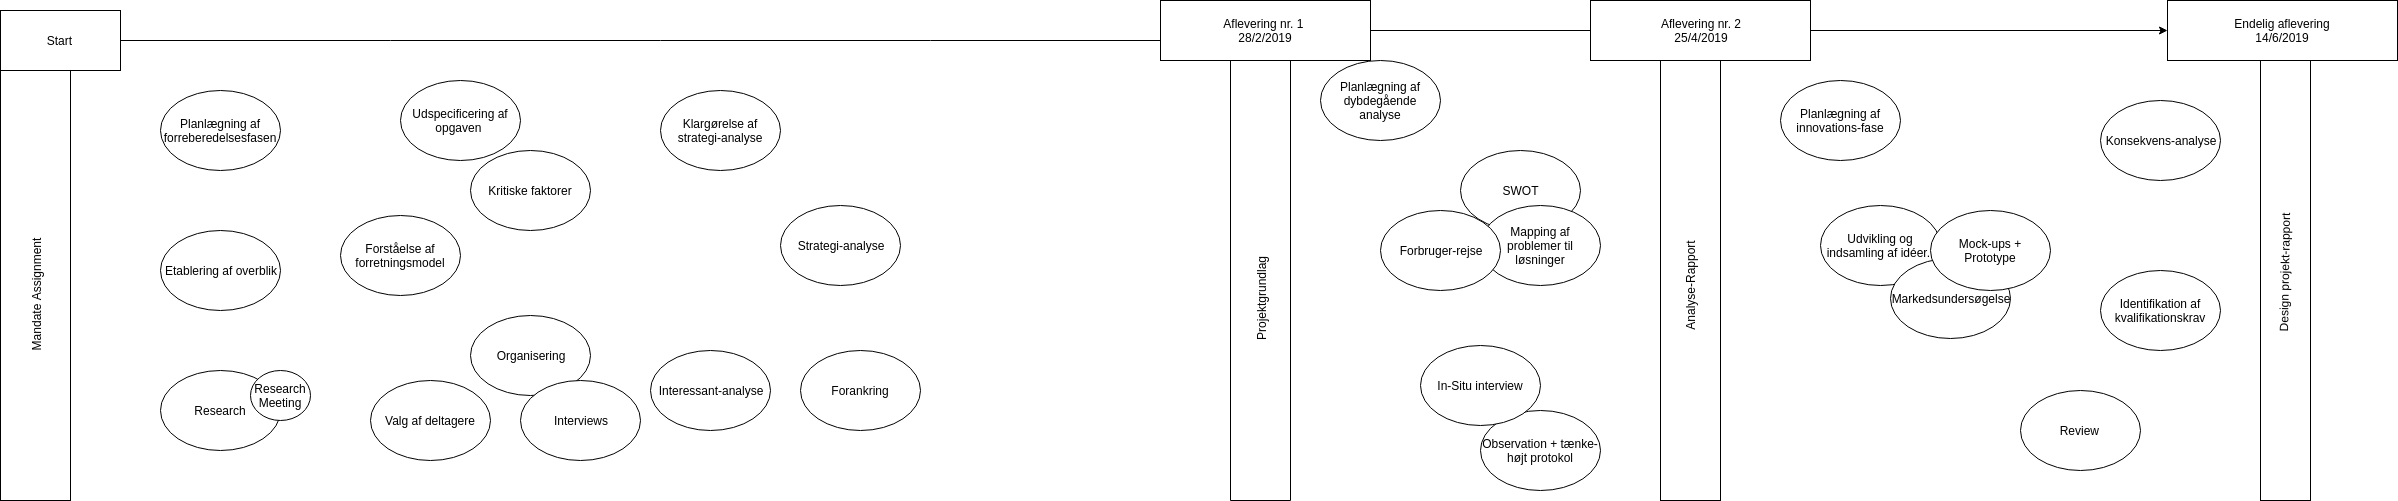
\includegraphics[width=1.2\textwidth, height=6cm]{Materials/Baseline}
	\caption{Udarbejdet baseline}
\end{figure}
Region Sjælland har et strategisk ønske om it systemet skal være gennemtestet samt at opnå fuld tilgængelighed blandt læger og patienter. Af denne årsag ønsker vi at lave en markedsundersøgelse for at finde inspiration. Hertil vil vi benytte os af SWOT-analysen til at visualisere hvorledes analysens elementer vægtes.\\
Som led i regionens strategi om at klinikere skal have overblik over relevante data og aftaler, vil vi arrangere insitu-interview, hvor vi kortlægger hvilke data der er relevante. Insitu-interview vil ligeledes også være relevante ift. patienter og behandlere, for at vi kan nedbringe konsultation- og behandlingstid.\\
Generelt ønsker både regionen og patienter at kunne udføre flere opgaver gennem selvbetjening, hvilket projektet vil arbejde sig hen imod.  
